\documentclass{beamer}

% === AUTOR === (((
\author{\textit{Por Erick I. Rodríguez Juárez.}}
% )))

% === PAQUETES === (((
% \usepackage{makeidx}
% \usepackage{xltxtra}
\usepackage{amsfonts}
\usepackage{amsmath}
\usepackage{amssymb}
% \usepackage{fullpage}
\usepackage{tikz}
\usetikzlibrary{arrows.meta}
\usepackage{graphicx}
% )))

% === TIPOGRAFÍA === (((
% \setmainfont[
  % BoldFont       = bodonibi,
	% ItalicFont     = Century modern italic2.ttf,
	% BoldItalicFont = bodonibi,
	% SmallCapsFont  = lmromancaps10-regular.otf
% ]{Century_modern.ttf}
% )))

% === COMANDOS === (((
% \newcommand{\dis}{\displaystyle}
% \newcommand{\qed}{\hspace{0.5cm}\rule{0.16cm}{0.4cm}}
% \newcommand{\operator}[1]{\mathop{\vphantom{\sum}\mathchoice
% {\vcenter{\hbox{\huge $#1$}}}
% {\vcenter{\hbox{\Large $#1$}}}{#1}{#1}}\displaylimits}
% \newcommand{\suma}{\operator{
\includegraphics[scale=0.09]{FOTOS/Sigma.png}}}
% \setlength{\parindent}{0mm}
% )))

% === ITALICA EN ENTORNO MATEMÁTICO === (((
% \DeclareSymbolFont{italics}{\encodingdefault}{\rmdefault}{m}{it}
% \DeclareSymbolFontAlphabet{\mathit}{italics}
% \ExplSyntaxOn
% \int_step_inline:nnnn { `A } { 1 } { `Z }
 % {  \exp_args:Nf \DeclareMathSymbol{\char_generate:nn{#1}{11}}{\mathalpha}{italics}{#1} }
% \int_step_inline:nnnn { `a } { 1 } { `z } {  \exp_args:Nf \DeclareMathSymbol{\char_generate:nn{#1}{11}}{\mathalpha}{italics}{#1}}
% \ExplSyntaxOff
% )))

\begin{document}

\frame{\titlepage}

\section{Movimiento Vibratorio de Sistemas Mecánicos.} % (((
\begin{frame}[t]
	\frametitle{Movimiento Vibratorio de Sistemas Mecánicos.}
	Suponga una masa \(m\) unida a un resorte flexible colgado sobre un soporte rígido. La distancia de alargamiento dependerá de la masa. Según la Ley de Hooke, el resorte mismo ejerce una fuerza de restitución opuesta a la dirección de alargamiento y proporcional al dicho alargamiento \(S\), es decir:
	\[
		F=kS \;,\; k = \mbox{constante del resorte.}
	\]
	\begin{figure}[ht]
		\centering
		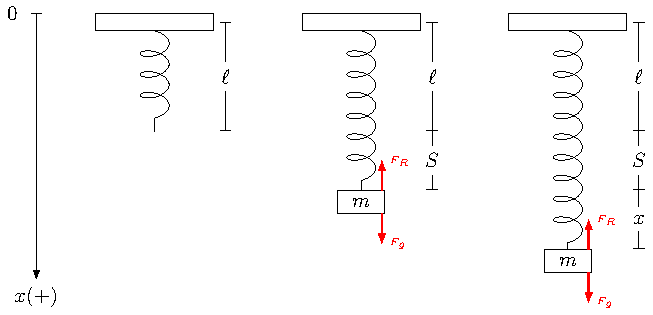
\includegraphics[width= 0.8 \linewidth]{IMAGENES/1/tikz.pdf}
	\end{figure}
\end{frame}

\begin{frame}[t]
	\begin{columns}
		\column{0.3\textwidth}
		Equilibrio
		\[
			\begin{array}{rcl}
				F_g-F_R & = & 0 \\
				F_g-kS & = & 0 \\
				\iff mg = kS.
			\end{array}
		\]
		\column{0.3\textwidth}
		Movimiento
		\[
			\begin{array}{rcl}
				F_T & = & F_g-F_R \\
				F_T & = & mg - k(S+x) \\
				F_T & = & mg - kS-kx \\
				F_T & = & -kx.
			\end{array}
		\]
	\end{columns}
\end{frame}

\begin{frame}[t]
	\begin{block}{}
		Por la \(2^{da}\) Ley de Newton \(F_T = ma = m \dfrac{dv}{dt} = m \dfrac{d^2x}{dt^2}\). Luego, igualando \(F_T = m \dfrac{d^2x}{dt^2} = -kx\), \(k,m >0\),
		\[
			\iff m \dfrac{d^2x}{dt^2} +kx =0 \iff \dfrac{d^2x}{dt^2} + \underbrace{\dfrac{k}{m}} _{w^2 = k/m >0}  x =0
		\]
		Luego, la ecuación que describe el movimiento de \(m\) está dada por
		\begin{center}
			\color{red} \fbox{\color{black} \(\dfrac{d^2x}{dt^2} + w^2x =0\)} \\
			\footnotesize E.D. para describir el Movimiento Armónico Simple.
		\end{center} 
		Resolvemos la E.D. usando la ecuación característica \(m^2+w^2=0 \iff m^2=-w^2 \iff m_{1,2} = \pm iw\), \(\alpha =0\), \(\beta =w\).
	\end{block}
\end{frame}
% )))

\end{document}
